\documentclass{article}

\usepackage{amsmath, amsthm, amssymb, amsfonts}
\usepackage{thmtools}
\usepackage{graphicx}
\usepackage{setspace}
\usepackage{geometry}
\usepackage{float}
\usepackage{hyperref}
\usepackage[utf8]{inputenc}
\usepackage[english]{babel}
\usepackage{framed}
\usepackage[dvipsnames]{xcolor}
\usepackage{tcolorbox}
\usepackage{textcomp}
\usepackage{listings} 


\colorlet{LightGray}{White!90!Periwinkle}
\colorlet{LightOrange}{Orange!15}
\colorlet{LightGreen}{Green!15}

\newcommand{\HRule}[1]{\rule{\linewidth}{#1}}

\declaretheoremstyle[name=Theorem,]{thmsty}
\declaretheorem[style=thmsty,numberwithin=section]{theorem}
\tcolorboxenvironment{theorem}{colback=LightGray}

\declaretheoremstyle[name=Proposition,]{prosty}
\declaretheorem[style=prosty,numberlike=theorem]{proposition}
\tcolorboxenvironment{proposition}{colback=LightOrange}

\declaretheoremstyle[name=Principle,]{prcpsty}
\declaretheorem[style=prcpsty,numberlike=theorem]{principle}
\tcolorboxenvironment{principle}{colback=LightGreen}

\setstretch{1.2}
\geometry{
    textheight=9in,
    textwidth=5.5in,
    top=1in,
    headheight=12pt,
    headsep=25pt,
    footskip=30pt
}

\begin{document}

\title{ \normalsize \textsc{}
		\\ [2.0cm]
		\HRule{1.5pt} \\
		\LARGE \textbf{\uppercase{Fashion Attributes Classification Challenges}
		\HRule{2.0pt} \\ [0.6cm] \LARGE{AI6126 Project 1} \vspace*{5\baselineskip}}
		}
\date{2024 - March - 29}
\author{\textbf{Riemer van der Vliet} \\ 
		G2304212K}

\maketitle

\newpage

\section{Introduction}

This report outlines the methodology and findings of the Fashion Attributes Classification Challenge, an individual endeavor focused on leveraging machine learning to categorize fashion images by attribute. Employing a dataset of 6,000 images, this project distinguishes itself through the use of Vision Transformers (ViT). The objective is to accurately predict multiple attribute labels for each image, a task that demands a model with nuanced understanding of the dataset. Particularly as this dataset is heavily unbalanced. 

\subsection{The dataset}

Fashion Attributes Classification Challenge dataset comprises 6,000 images, thoughtfully partitioned into sets of 5,000 for training and 1,000 for validation. This rich dataset is annotated with 26 distinct attribute labels spread across six primary categories, framing a complex multi-label classification scenario. Each image is tagged with six attributes, one from each category. Some examples can be seen in figures~\ref{fig:four_images}.


\begin{figure}[ht]
    \centering
    \begin{minipage}[b]{0.2\linewidth}
        \centering
        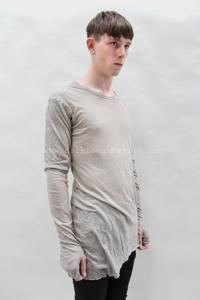
\includegraphics[width=\linewidth]{imgs/00000.jpg}
    \end{minipage}
    \hfill
    \begin{minipage}[b]{0.2\linewidth}
        \centering
        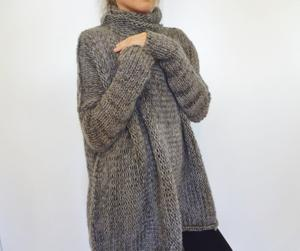
\includegraphics[width=\linewidth]{imgs/00001.jpg}
    \end{minipage}
    \hfill
    \begin{minipage}[b]{0.2\linewidth}
        \centering
        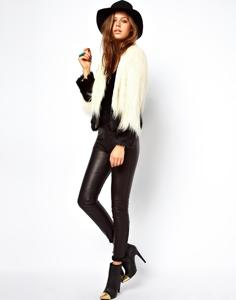
\includegraphics[width=\linewidth]{imgs/00002.jpg}
    \end{minipage}
    \hfill
    \begin{minipage}[b]{0.2\linewidth}
        \centering
        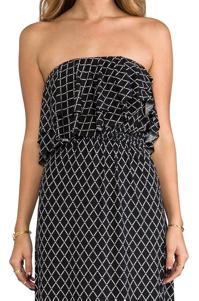
\includegraphics[width=\linewidth]{imgs/00003.jpg}
    \end{minipage}
    \caption{First 4 entries of the dataset.}
    \label{fig:four_images}
\end{figure}


The dataset is regularized with a simple transformer as can be seen in the code in \href{https://github.com/Riemer1818/AI6126-AdCV-Proj1/blob/main/code/finalCode.py}{The code} and in code block~\ref{fig:transform_code}. Where a RandomVerticalFlip is added to increase the number of datapoints, but no RandomHorizontalFlip is added as this is not representative of the test set. 

\begin{figure}[ht]
    \centering
    \begin{lstlisting}[language=Python]
    transform = transforms.Compose([
        transforms.Resize((224, 224)),
        transforms.ToTensor(),
        transforms.Normalize((0.5, 0.5, 0.5), (0.5, 0.5, 0.5)),
        transforms.RandomVerticalFlip(p=0.5)
    ])
    \end{lstlisting}
    \caption{Code snippet for dataset transformation}
    \label{fig:transform_code}
\end{figure}

\subsubsection{Weight regularization}
Addressing the challenge of dataset imbalance, a weight regularization strategy has been implemented. You can see the relative weights as they are computed in figure~\ref{fig:weight_distribution}. This approach aims to normalize the representation of classes within the model, mitigating the skewness caused by varied class frequencies. As such when calculating the loss function the weights are used to balance the loss function.

\begin{figure}[ht]
    \centering
    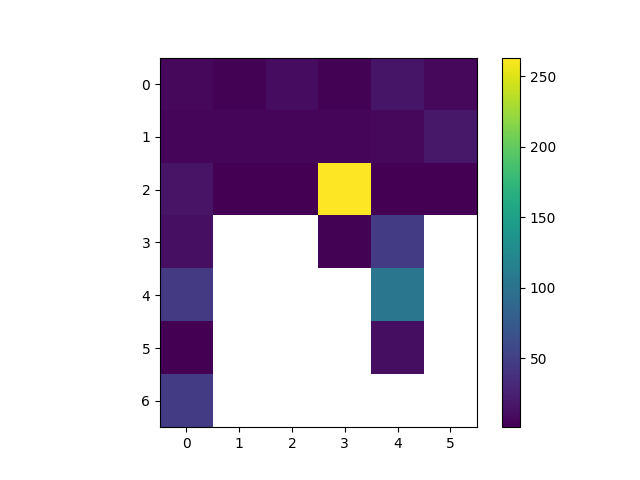
\includegraphics[width=0.8\linewidth]{imgs/distribution.png}
    \caption{Weight distribution of classes}
    \label{fig:weight_distribution}
\end{figure}


\subsubsection{Loss function}

Because of the weight imbalance as mentioned earlier and the multi-label classification task, a weighted binary cross-entropy loss function has been employed. This function is designed to assign different weights to each class based on their frequency, ensuring that the model learns to predict all classes effectively. This approach is crucial for optimizing the model's performance and enhancing its ability to classify fashion attributes accurately.

\subsection{Description of model}

In training the model I have taken particular note in making sure the model was able to capture subclasses within the dataset as such we will employ a Multitaskhead with some shared Relu layers with dropout and some task specific layers 

\subsubsection{ViT}

The Vision Transformer (ViT) model marks a paradigm shift from traditional convolution neural networks to a transformer-based approach that treats image patches as sequences for classification tasks. This model capitalizes on the transformer's ability to capture long-range dependencies which might work well in a dataset with big differences within image projection. The precise model used is a \href{https://huggingface.co/google/vit-base-patch16-224-in21k}{vit-base-patch16-224-in21k} from Hugging Face. Notably the author did not read the documentation of this model and accidentally used a model trained on 21k images opposed to the required 10k. 

\subsubsection{MultiTaskHead}

At the heart of our model lies the MultiTaskHead module, engineered to concurrently predict multiple attribute labels. This functionality is vital for the Fashion Attributes Classification Challenge, ensuring the model's efficiency and efficacy in multi-label classification. The module's architecture, integrated within a pre-trained ViT framework, demonstrates a robust approach to handling the intricacies of fashion attribute classification. The printed model can be seen in the appendix~\ref{app:model}.

\subsubsection{Model Architecture}
The model employs a pre-trained Vision Transformer (ViTForImageClassification) as its backbone, featuring an intricate network of embeddings, encoders, and a MultiTaskHead for classification. The encoder, composed of 12 transformer layers, processes sequences of image patches through a series of self-attention mechanisms and feed forward networks. This is followed by a MultiTaskHead classifier, which includes shared layers for general feature processing and task-specific layers designed to output predictions for each attribute category. The structure and parameterization of this model underscore its potential to capture and interpret the complex patterns inherent in fashion imagery, providing a detailed and nuanced understanding of fashion attributes. 


\section{Results}

figure~\ref{fig:TrainingLoss} shows the training loss during training, while figure~\ref{fig:ShortTrainLoss} illustrates the model training with a high learning rate. This exploration methods indicated that a more optimal solution would be somewhere in the middle. As can be seen in the training loss graph in figure~\ref{fig:TrainingLoss} the training is smooth up to this point but seems to stagnate. The full training sets can be found in~\ref{tab:model_parameters}. Where I have employed crossing to quickly pinpoint optimal parameters. 

From this I conclude that my loss function is not able to accuracy project the loss. This is also visible in the validation loss graph in figure~\ref{fig:ValidationLoss}. The validation loss is not decreasing as expected. This is a clear indication that the model is not learning as expected.

\begin{table}[ht]
    \centering
    \begin{tabular}{ccccc}
        \hline
        \textbf{Epochs} & \textbf{Learning Rate} & \textbf{Dropout Rate} & \textbf{Average Class Accuracy} & \textbf{Total Accuracy} \\
        \hline
        10 & 0.0031 & 0.22 & 0.23 & 0.52 \\
        20 & 0.00031 & 0.22 & 0.58 & 0.75 \\
        20 & 0.00031 & 0.3 & 0.56 & 0.72 \\
        20 & 0.0004 & 0.22 & 0.54 & 0.72 \\
        50 & 0.000031 & 0.22 & 0.54 & 0.6 \\
        \hline
    \end{tabular}
    \caption{Model Training Parameters: Layers Unfrozen: 1, Epochs, Learning Rate, Dropout Rate, Average Class Accuracy, Total Accuracy. Batch Size: 32}
    \label{tab:model_parameters}
\end{table}

\begin{figure}[H]
    \centering
    \begin{minipage}[b]{0.45\textwidth}
        \centering
        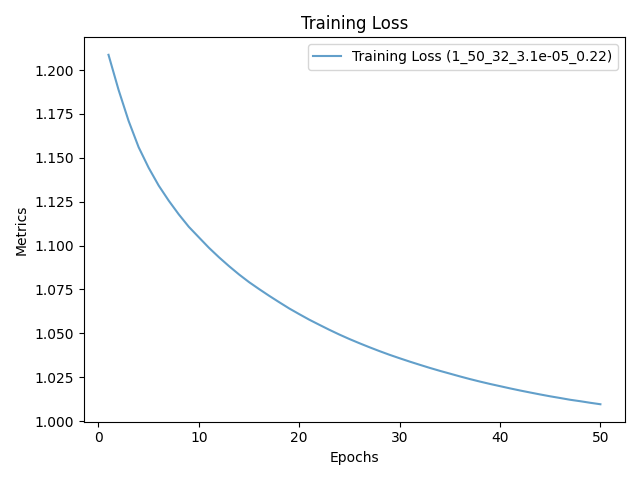
\includegraphics[width=\textwidth, height=5cm]{imgs/long_train_loss.png}
        \caption{Here the model is trained over 50 epochs with low learning rate. The image shows the loss during training.}
        \label{fig:LongTrainLoss}
    \end{minipage}
    \hfill
    \begin{minipage}[b]{0.45\textwidth}
        \centering
        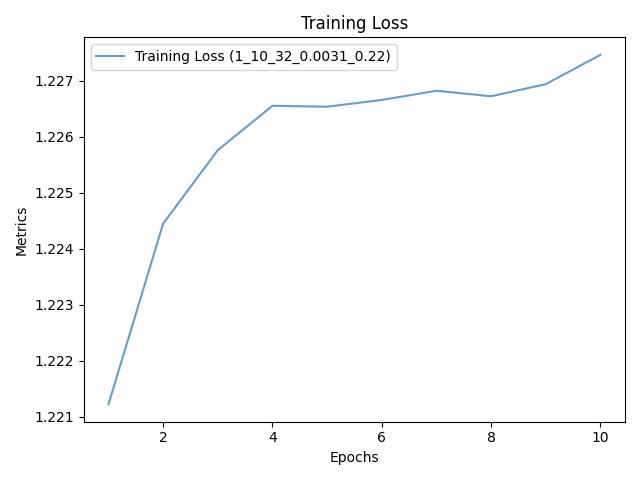
\includegraphics[width=\textwidth, height=5cm]{imgs/short_train_loss.png}
        \caption{Here the model is trained over 10 epochs with high learning rate.}
        \label{fig:ShortTrainLoss}
    \end{minipage}
\end{figure}

\begin{figure}[H]
    \centering
    \begin{minipage}[b]{0.45\textwidth}
        \centering
        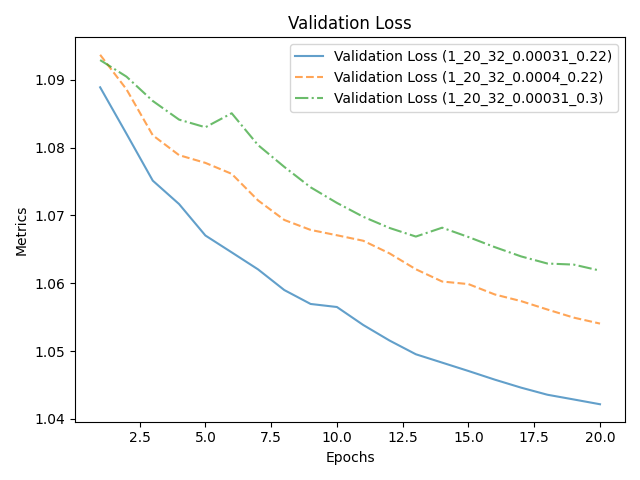
\includegraphics[width=\textwidth, height=5cm]{imgs/Validation_loss3.png}
        \caption{Validation Loss during Training}
        \label{fig:ValidationLoss}
    \end{minipage}
    \hfill
    \begin{minipage}[b]{0.45\textwidth}
        \centering
        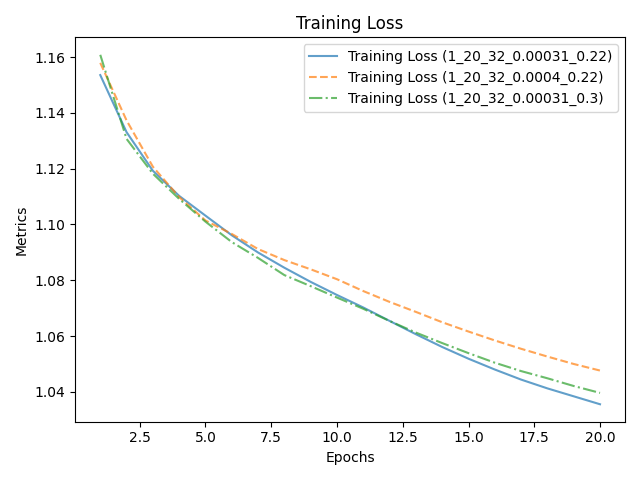
\includegraphics[width=\textwidth, height=5cm]{imgs/Training_loss3.png}
        \caption{Training Loss during Training}
        \label{fig:TrainingLoss}
    \end{minipage}
\end{figure}

\begin{figure}[H]
    \centering
    \begin{minipage}[b]{0.45\textwidth}
        \centering
        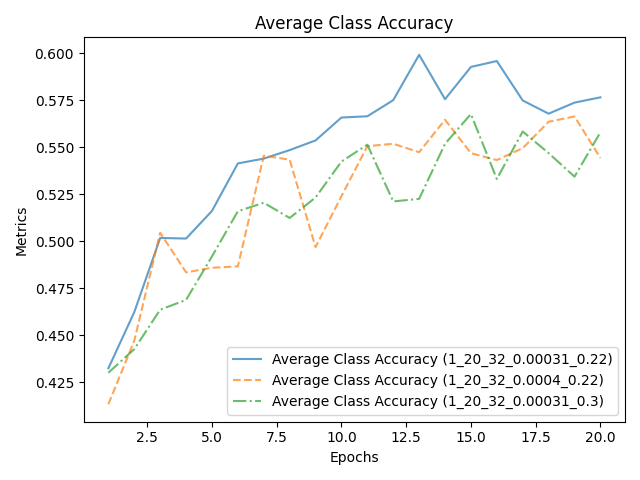
\includegraphics[width=\textwidth, height=5cm]{imgs/Average_accuracy.png}
        \caption{Average Accuracy during Training}
        \label{fig:AverageAccuracy}
    \end{minipage}
    \hfill
    \begin{minipage}[b]{0.45\textwidth}
        \centering
        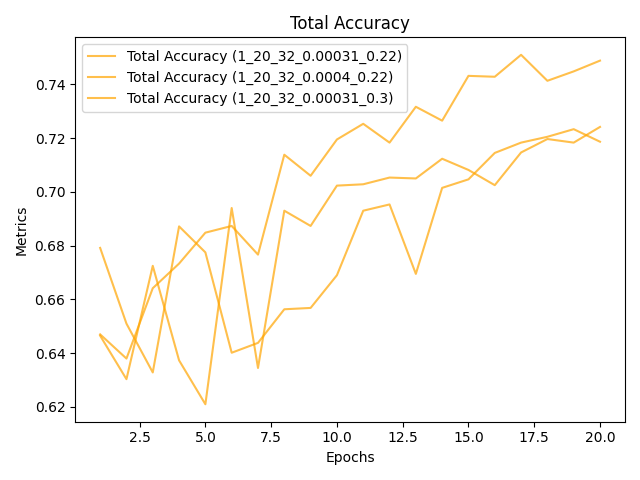
\includegraphics[width=\textwidth, height=5cm]{imgs/Total_accuracy.png}
        \caption{Total Accuracy during Training}
        \label{fig:TotalAccuracy}
    \end{minipage}
\end{figure}


\section{Discussion}

Based on the training and validation loss graphs shown in Figures\ref{fig:LongTrainLoss} and\ref{fig:ShortTrainLoss}, it is evident that the model's performance is not satisfactory. The training loss seems to stagnate, indicating that the model is not learning as expected. Similarly, the validation loss does not decrease as expected, further confirming that the model is not performing optimally. It is clear that the chosen ViT (Vision Transformer) model is not able to effectively capture the complex patterns inherent in fashion imagery. This might due to using a model trained on 21k images instead of the required 10k images, which might not have good capabilities to represent a smaller dataset. 

Despite the suboptimal performance, the model achieved the best results with the parameters: 1 layer unfrozen, 20 epochs, batch size of 32, learning rate of 0.00031, and dropout rate of 0.22. These parameters were selected based on a combination of experimentation and cross-validation to find a balance between model performance and computational efficiency. However, it is important to note that these parameters still did not yield satisfactory results.

Further investigation is required to determine the optimal parameters for the model. However, it is worth noting that training a ViT model requires substantial computational resources, which are currently unavailable to me. This limitation hinders the ability to conduct extensive testing and parameter tuning as well as retrain the model using a 10k variant. 

Despite the suboptimal performance, the model achieved a final test score of 0.57721. The model was unable to express the data better and trials with optimizers such as \href{https://optuna.org/}{Optuna} did not yield better results (not shown in report).

In conclusion, the current model's performance falls short of expectations. The limitations of the chosen ViT model and the lack of computational resources hindered the ability to achieve optimal results. Further research and experimentation are necessary to overcome these challenges and improve the model's performance. 

To reproduce the results please have a look at the code in the \href{https://github.com/Riemer1818/AI6126-AdCV-Proj1/blob/main/code/finalRunner.ipynb}{finalRunner} and generally at the \href{https://github.com/Riemer1818/AI6126-AdCV-Proj1/}{github repository}. The model weights for the best performing model can be found under \texttt{./content/models/1\_20\_32\_0.00031\_0.22/1\_20\_32\_0.00031\_0.22\_best\_model.pth}


\newpage

\section{References}
\bibliographystyle{IEEEtran}
\bibliography{References.bib}

\itemize{
    \item Hugging Face - \href{https://huggingface.co/google/vit-base-patch16-224-in21k}{ViT Model}
    \item Optuna - \href{https://optuna.org/}{Optuna}
    \item ChatGPT - \href{https://www.openai.com/chatgpt/}{ChatGPT}
    \item Co-pilot - \href{https://copilot.github.com}{Co-pilot}
}

\section{Appendix}

\begin{figure}[ht]
    \centering
    \begin{lstlisting}[language=TeX]
======================================================================
Layer (type:depth-idx)                        Param #
======================================================================
->ViTForImageClassification: 1-1              --
|    ->ViTModel: 2-1                          --
|    |    ->ViTEmbeddings: 3-1                (742,656)
|    |    ->ViTEncoder: 3-2                   (85,054,464)
|    |    ->LayerNorm: 3-3                    (1,536)
|    ->MultiTaskHead: 2-2                     --
|    |    ->Sequential: 3-4                   2,886,656
|    |    ->ModuleList: 3-5                   26,650
======================================================================
Total params: 88,711,962
Trainable params: 2,913,306
Non-trainable params: 85,798,656
======================================================================
    \end{lstlisting}
    \caption{Code snippet representing the layer structure of the ViT model.}
    \label{app:model}
\end{figure}

\end{document}
